\documentclass[11pt,a4paper]{article}
\usepackage{graphicx}
\usepackage[numbers]{natbib}
\usepackage[hyphens]{url}
% \usepackage[german]{babel}
\usepackage[british]{babel}
\usepackage[utf8]{inputenc} %für Umlaute äüöß
\usepackage{array}
\graphicspath{{images/}}

\begin{document}


\begin{titlepage}
\setlength{\parindent}{0pt} %remove indent at new paragraph
\begin{center}

% PROFESSOR, FACULTY AND UNIVERSITY
\small{Prof. Dr. Fabian J. Sting \\
Department of Supply Chain Management – Strategy and Innovation \\
University of Cologne\\}
\vspace{20mm}

% TOPIC NAME
\Huge{SpaceX Operations Strategy Analysis}
% SUBTITLE
% \small{}

\vspace{10mm}
\begin{figure}[!h]
    \centering
    
\includegraphics[width=0.7\textwidth]{siegel.png}
\end{figure}

\vspace{10mm}

% AUTHORS
\small{
Pascal Brokmeier (5868483) \\
Joel Charlier (7334647) \\
Christian Hovestadt (5589444) \\
Philipp Jann (7341343) \\
}

\vspace{10mm}
\today
\pagenumbering{gobble}
\end{center}
\end{titlepage}

% THIS IS THE BEGINNING OF THE FILE TEXT
\newpage
\pagenumbering{arabic}
\section{Introduction}\label{introduction}
The airspace-launching-company SpaceX has redefined launch system industries expectations within the last decade. With their innovative products, especially regarding reusability, they are able to cut costs significantly, disrupting  a former governmental-institution dominated and cost-inefficient market towards a fully private, profit-based business. SpaceX’s market success was only possible by redefining established market dynamics and implementing an innovative operations strategy. This report discusses previously existent structures in the rocket market, SpaceX’s disruptive strategy  and competitive advantages as well as responses of competitors.
\section{Background}\label{background}
% \subsection{Development of the rocket industry}

The Space Race of the 60s and 70s, triggered by the Soviet Union sending the first human into space, created the market of spaceflight. At that time, getting the lead in space exploration was a prestigious battle between the Soviets and the United States, which entailed high financial support from the government for the respective institution \cite{scs57}. Since the end of the space race around 1970 only few cost reductions were achieved and the lower earth orbit transportation cost remained stable between 10,000 and 25,000USD/kg. A typical rocket consists of two to five stages only used to accelerate the rocket during the start. They cannot be landed safely and therefore can not be used again. In 2007, the German Society for Aeronautics and Astronautics (DGLR) claimed that the inevitable next step to reduce cost is to produce reusable rockets and hence to decrease the cost of rocket launches dramatically \cite{scs58}.
\subsection{ Current market situation}\label{current-market-situation}

Excluding the US-market, the most important players in the industry of rocket manufacture on the global market are the European company Arianespace, the Russian company Khrunitchev and the Chinese CNSA.



\begin{figure}[!h]
    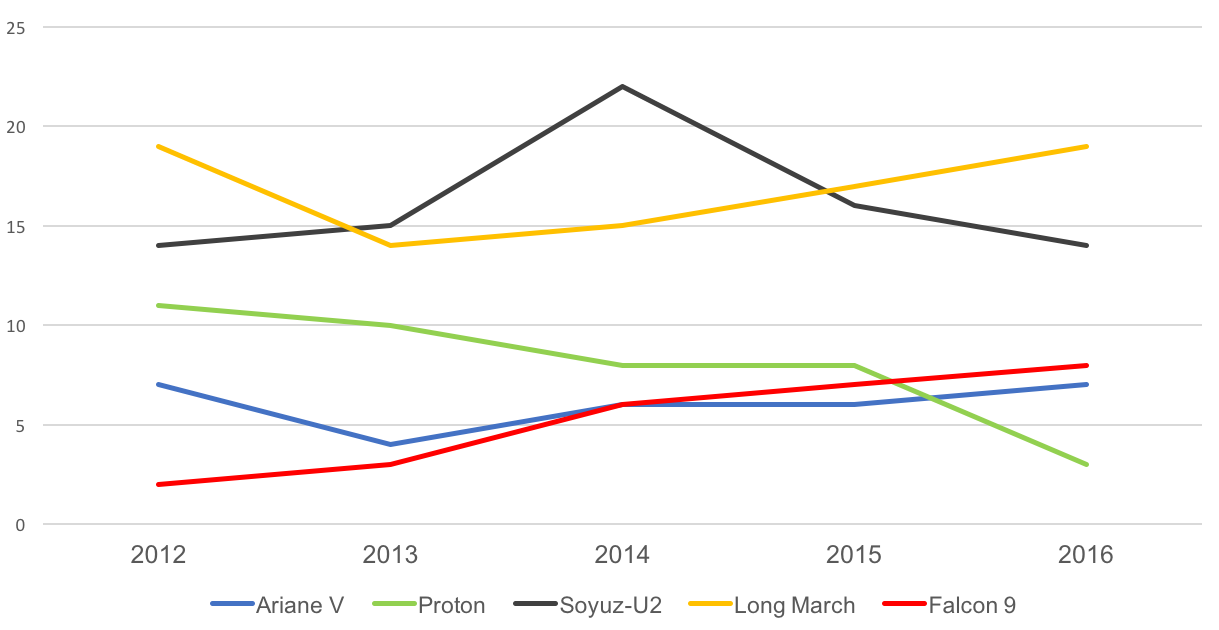
\includegraphics[width=1.0\textwidth]{image1.png}
    \centering
    \caption{Launches per year from 2012-2016 \cite{scs59}, \cite{scs61}, \cite{scs61},\cite{scs68}, \cite{scs69}}
    \label{figure1}
\end{figure}

Figure \ref{figure1} above shows the five most launched rockets between 2012 and 2016. Although Arianespace does not execute the most launches, they’ve been market leader in commercial launches in 2014 and 2015 \cite{scs64}. A launch of a satellite with the Ariane V launch system costs Arianespace around \$137Mio, according to former CEO Le Gall \cite{scs62}. Another market player is the China National Space Cooperation (CNSC), which mainly uses the Long March 3B. CNSC plans to reduce their cost by replacing the highly toxic hydrazine propellant with a mix of kerosene and liquid oxygen for their new Long March 5,6 and 7 \cite{scs63}.
Two further important rockets are the Russian rockets Proton and Soyuz. Proton is manufactured by Khrunichev and can carry up to 6,300kg into geosynchronous transfer orbit (GTO) \cite{scs70}. The Russian Soyuz-U2 rocket belongs to the R-7 family, which is the most launched rocket family worldwide. The Soyuz-U2 rocket can launch up to 2,900kg into GTO \cite{scs73} and is also modified and launched by Arianespace \cite{scs74}.

The conditions on the US-market are special, since the government does not want to be dependent on foreign companies for their space missions. It has to be differentiated between governmental mandatories, given by the NASA and the airforce and the commercial market, where the biggest launch providers are United Launch Alliance (ULA) and SpaceX, a private company founded by entrepreneur Elon Musk. The NASA uses rockets of other companies for their launches, while they are developing their own new rocket, the Space Launch System, since 2011 \cite{scs71}. A big problem in this process are the "cost-plus contracts" negotiated by the US-government with their suppliers and which require the NASA to pay for all incurring cost plus a formula-based profit on top of the agreed predicted cost \cite{scs72}. This leads to high prices since the suppliers have no incentive to reduce their expenses. NASA-used rockets are mainly Delta II, built by ULA, and Falcon 9 by SpaceX.


\subsection{SpaceX}
SpaceX was founded in 2002 by the entrepreneur Elon Musk, founder of Tesla and co-founder of PayPal. The company headquarter in Hawthorne, California has currently more than 5,000 employees \cite{scs76}. Their market share in 2017 is approximately 45\% and is predicted to be 60\% in 2018 \cite{scs64}.
\section{Operations at SpaceX}\label{operations-at-spacex}
% \subsection{Products}\label{products}
SpaceX focuses on only two types of rockets: The \emph{Falcon 9} and the \emph{Falcon Heavy} for different payload quantities \cite{scs20}. They apply the swiss-army-knife-strategy, as these rockets are the same regardless of the mission they will fly, e.g. low-orbit flights or resupply flights to the international space station \cite{scs33}. The two rockets share a great deal of component commonality and additionally, commonalities are maximized within each rocket:  For example, the fuel tanks of the second stage are a shorter version of the first-stage tanks, which allows the use of the same tools, materials and manufacturing processes \cite{scs33}.
The Dragon spaceship can me mounted to the top of every Falcon rocket. Again, SpaceX unifies multiple functions in one product, as the Dragon is designed to carry humans as well as cargo \cite{scs19}.
These highly standardized products aggregate the demand and reduce the need for safety stock significantly.
\subsection{ Reusability of Stage 1 initiative}\label{reusability-of-stage-1-initiative}

In essentially every other transport mode, the vehicle can be reused for several trips. SpaceX COO Gwynne Shotwell argued in front of a committee in 2015 that the lack of reuse of rockets in space travel is “akin to throwing away an airplane after every leg of a trip” \cite{scs21}. SpaceX intends to change this paradigm by landing their first-stage rocket boosters after it detaches from the second stage and reusing them for multiple trips.
This plan was followed through with several landings in 2015 and 2016 both on land and on drone ships floating in the ocean. “The world’s first reflight of an orbital class rocket” was then performed in March 2017 \cite{scs34} and all flights of 2017 that were intended for recovery have successfully been recovered. This made SpaceX the first company to reuse rocket hardware since NASA’s space shuttle program \cite{scs15}.
Reusability reduces the price for flying again significantly as can be seen in Table \ref{table}.





This price reduction for Falcon 9 and Heavy above includes a 50\% passalong of savings through stage 1 reuse to the customer and 50\% of the savings being kept by SpaceX for further investments in R&D meaning they still have a large buffer to further reduce the price to stay competitive or to put further pressure on the market competitors.
\cite{scs15}

\begin{table}[]
\renewcommand{\arraystretch}{1.3}
\begin{tabular}{l|l|l|l}
    \hline
                                 & Payload (tons) & Price (\$Mio) & Price (\$/kg) \\
Falcon 9                         & 22.8           & 62            & 2719          \\
Atlas                            & 18.8           & 163           & 8670          \\
Falcon 9 with reuse              & 22.8           & 43.3          & 1899          \\
Falcon Heavy                     & 63.8           & 90            & 1410 \\
\hline
\end{tabular}
\centering
\caption{Comparison of US government certified launch-vehicles \cite{scs24, scs15, scs20}}
\label{table}
\end{table}

\subsection{Processes}\label{processesn}
SpaceX unifies the traditional roles of launch operations provider, rocket manufacturer and rocket engine supplier, which helps with cost reduction and reduces the dependency on external suppliers or foreign manufacturers. This was an argumentative advantage over ULA, who sourced the engine for their rockets from russian manufacturers before signing a deal with Blue Origin recently due to a ban on non US sourced rockets for national security satellite launches \cite{scs31}. Therefore, SpaceX emerged as the only US-based provider for launching satellites, independent from foreign engines. To cover the resulting shift in demand, the company attained several process advantages, allowing rapid manufacturing and deployment of launch vehicles:

With a manufacturing floor plan designed for engine mass production, SpaceX builds 70\% of their rockets in their plant in California. This is especially helpful as each Falcon 9 uses 9 Merlin engines in a cluster, leading to economies of scale in producing low-cost launch vehicles that can handle up to two engine failures while still succeeding in payload delivery.
Further standardization in manufacturing processes is achieved by building each Falcon 9 identically, regardles of the mission type (GSO, low earth orbit or ISS missions) and constructing Stage 1 and Stage 2 engines with only minor differences in specifications.
Current production capability allows for up to forty stage 1 cores annually which, combined with the reuse abilities, will allow SpaceX to offer several flights per month with prices that are much lower than current market standards \cite{scs33} and therefore will increase demand drastically as many business models can be reevaluated with new pricing standards \cite{scs33}.

Another interesting factor for low operation cost of research can be attributed to a young workforce of highly motivated and non-unionized recent university graduates which are willing to work large amounts of unpaid overtime \cite{scs4}. SpaceX has repeatedly stated its main goal is repeated missions to Mars and they often use a rotating depiction of the planet turning green to reference to their vision of terraforming the planet \cite{scs6}.
% REACTIONS
\section{Reactions by competition}\label{reactions-by-competition}
SpaceX’s major market advantage, lowering rocket launch costs drastically, led to significant market share redistribution and a price-lowering wave within the global rocket-launch-market.
\subsection{Arianespace}\label{arianespace}
Their main competitor for commercial launches, French-based company Arianespace, reacted by decoupling its established per-kilogram pricing policy for lighter satellites to remain competitive \cite{scs41}. Not undervaluing the power of SpaceX’s disruptive technology, the company has decided to focus on its  major advantage compared to SpaceX: Reliability. CEO Stéphane Israel states, that new-build rockets are more reliable than reused ones, ensuring success of space missions. Nevertheless, Arianespace has announced to develop a new rocket, “Ariane 6”, by 2020, that is supposed to be around 50\% cheaper than existing models and whose costs shall be lowered on the long-term. Referring to reusability, Arianespace plans to reuse the 2nd stage rocket part as a satellite-tug in space \cite{scs44}. Moreover, major shareholder Airbus has invested venture capital into R&D-centers in silicon valley, operating detached of Arianespace, to force innovation via experimental power \cite{scs45}.
\subsection{United Launch Alliance}\label{ula}
Government-funded ULA might be the competitor most affected by SpaceX, as both companies are competing for commercial and governmental-funded US-market. After SpaceX’s market entry, ULA tried to cut costs drastically by thinning out their staffing level \cite{scs47}, which led them  to be twice as expensive in rocket launches as SpaceX, how US-Department of Defense budget requests revealed \cite{scs48}. The company wants to streamline their processes by dropping unnecessary tests. Additionally, rocket reusability plans were published: in their more cost efficient new rocket “Vulcan”, for which engine development is outsourced to US-based Blue Origin, first stage rocket engines shall be embedded in heat protection and come back to earth via parachute, being collected by helicopters \cite{scs47,scs49}. As SpaceX’s don't yet have a reliable enough track record, a requirement for US Departement of Defense contracts, ULA still wins major governmental contracts and remains competitive \cite{scs50}.
\subsection{Khrunichev}\label{khrunichev}
After commercial rocket launch-failures in 2014 and 2015, Khrunichev had problems to remain competitive, while SpaceX entered the market. While a financial rehabilitation program was implemented, Khrunichev responded to SpaceX’s price war by introducing two more cost-efficient versions of their Proton-rocket used for small and medium sized satellites at only slightly higher prices than SpaceX’s Falcon 9 \cite{scs51}. For its new rocket-family “Angara” Khrunichev has developed “Baikal Booster”, a reusable engine, that airplane-like flies back to its point of departure and therefore reduces costs significantly \cite{scs53}.
\subsection{Other competitors}\label{other-companies}
For completeness of information, two other organizations with future major market impact shall be mentioned: Firstly, Chinese state-owned organization CASTC, announcing a hybrid-rocket for mid-2030s, that can take-off from a usual landing strip and easily be relanded \cite{scs55}. Secondly, Jeff Bezos funded US-based company Blue Origin, who pursues a business model simliar to that of SpaceX. Blue Origin is already a major engine-developer and focuses on rocket launches with their new product “New Glenn”, whose 2nd stage will be largely reusable \cite{scs56}.
\section{Conclusion}\label{conclusion}
After cost-efficiency has not been the rocket industry’s main focus for decades, SpaceX is currently disrupting the market with its low-cost Falcon rockets. This competitive advantage was primarily achieved after great investments in the “Reusability of Stage 1 Initiative”, which allows rocket boosters to be reused for multiple journeys for the first time. Furthermore, a highly standardized rocket design and vertical process integration contribute to SpaceX’s success. After the majority of established competitors did not believe in the feasibility of SpaceX’s plans (at least not publicly), SpaceX is now years ahead of them in terms of technology.

\newpage
%Bibliography
\bibliographystyle{apalike}
\bibliography{sources}

\end{document}
